\section{Diagramme de planification temporel des tâches}
	Voir figure \ref{gantt}.
	
	\begin{figure}[htp]
		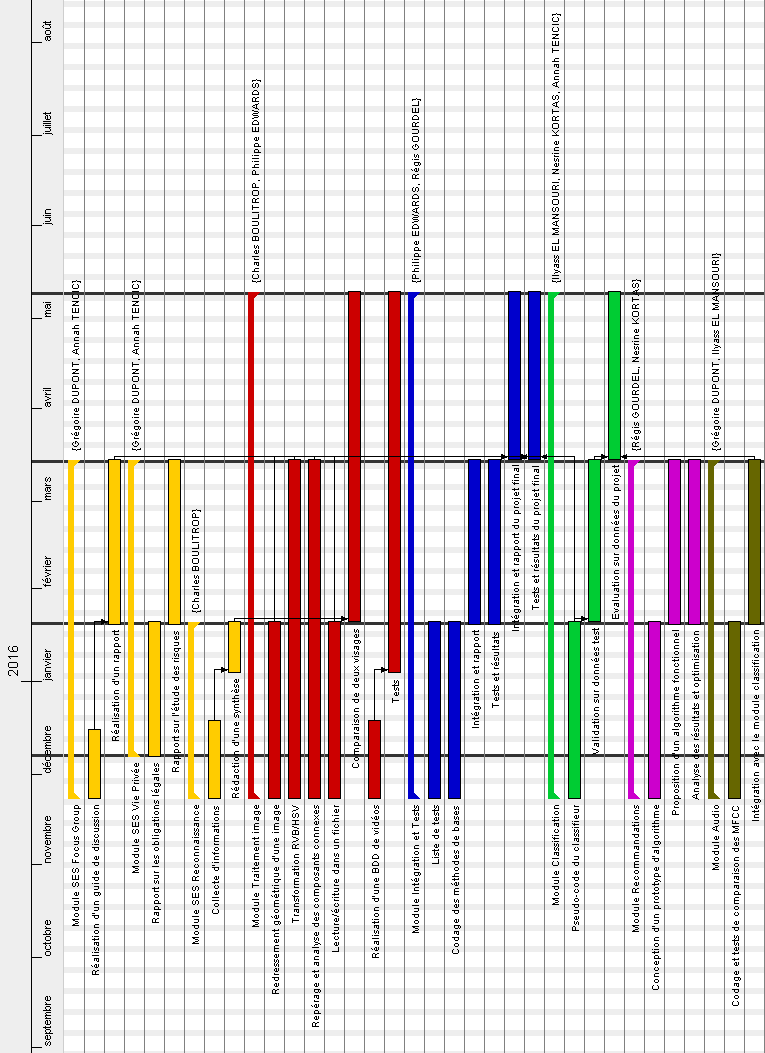
\includegraphics[scale=0.60]{images/gantt2.png}
		\caption{Diagramme chronologique de Gantt}
		\label{gantt}
	\end{figure}
		


\section{Répartition des élèves par module}
	\begin{tabular}{l|l|ccccccc}
		Nom module                   & Nom Expert & A. & N. & G. & I. & P. & C. & R. \\ % Les lettres étaient les initiales de nos prénoms...
		\hline
		Module 1 & Prénom Nom &    &\ct &    &    &    &    &\ct \\
		Module 2 & Prénom Nom &\ct &\ct &    &\ct &    &    &    \\
		Module 3 & Prénom Nom &\ct &    &\ct &    &    &    &    \\
		Module 4 & Prénom Nom &\ct &    &\ct &    &    &    &    \\
		Module 5 & Prénom Nom &    &    &    &    &    &\ct &    \\
		Module 6 & Prénom Nom &    &    &\ct &\ct &    &    &    \\
		Module 7 & Prénom Nom &    &    &    &    &\ct &\ct &    \\
		Module 8 & Prénom Nom &    &    &    &    &\ct &    &\ct
	\end{tabular}


\section{\textcolor{RoyalBlue}{Plans de test}}

	\setlongtables

\begin{longtable}{m{1.9cm}|m{3.9cm}|m{2.9cm}|m{2.9cm}|m{2.5cm}}
	\textbf{Module} & \textbf{Description du test} & \textbf{Entrée} & \textbf{Sortie attendue} & \textbf{Validation} \\
	\hline
	\endhead

	\textcolor{Green}{Image} &
		Test de fonctionnalité : extraction des paramètres en conditions normales &
		Ensemble réduit d'images de visages &
		Paramètres extraits &
		Voir annexe du module \\
	\hline

	\textcolor{Green}{Image} &
		Mesures de performance &
		Une prise (dix images) &
		Temps de calcul de environ 2 s &
		Le temps est satisfaisant.
		Dépend des performances de l'ordinateur. \\
	\hline

	\textcolor{Green}{Classification (images)} &
		Test de fonctionnalité : cas normal avec paramètres choisis &
		Paramètres correspondants à des visages &
		Émotions &
		Taux de succès de 70\% pour un test en validation croisée \\
	\hline

	\textcolor{Green}{Classification (images)} &
		Mesure de performance sur quelques entrées &
		Ensembles de paramètres types correspondants à des visages &
		Temps d'exécution : 1500 ms par prise, variable en fonction des performance de l'appareil. &
		Le temps obtenu est acceptable. \\
	\hline

	\textcolor{Green}{Classification (musiques)} &
		Test de fonctionnalité &
		Plusieurs musiques &
		Émotions associées aux musiques &
		Taux de réussite : 69\%. \\
	\hline

	\textcolor{Green}{Classification (musiques)} &
		Mesure de performance sur quelques entrées &
		Série de 60 musiques. &
		Temps d'exécution : 1500 ms. &
		Le temps est suffisant pour un usage classique, ceci n'étant réalisé que ponctuellement. \\
	\hline

	\textcolor{Green}{Image et classification} &
		Mesure de performance : temps total de reconnaissance de l'émotion &
		Ensembles d'images avec ou sans visage &
		Temps d'exécution 8152 ms &
		Temps acceptable pour cette application. \\
	\hline

	\textcolor{Green}{Audio MFCC} &
		Test de fonctionnalité &
		Ensemble de musiques &
		Moyenne quadratique par rapport à des résultats théorique. &
		Taux d'erreurs : 8\%. \\
	\hline

	\textcolor{Green}{Audio MFCC} &
		Test de performance &
		Ensemble de musiques &
		Temps d'exécution 2000 ms par musique. &
		Valeur un peu trop grande en cas de gros ajout mais passable. \\
	\hline
	
\end{longtable}


\section{Diagramme d’avancement des tâches}

	\subsection{Avancement au PAN 2}
	
	\begin{tabular}{lm{1.9cm}m{1.9cm}m{1.6cm}m{5.1cm}}
		Module & Avancement prévu (\%) & Avancement réel (\%) & Temps passé (h) & Description brève du travail effectué, analyse des écarts constatés \\
		\hline \hline
		Module 1 &
			30\% & 30\% & 18 h &
			Élaboration du plan de test, familiarisation avec le code, compilation et modification de quelques éléments graphiques. \\
		\hline
		Module 2 &
			50\% & 45\% & 20 h &
			Blablabla. \\
		\hline
		Module 3 &
			40\% & 40\% & 10 h &
			Blablabla. \\
		\hline
		Module 4 &
			40\% & 40\% & 10 h &
			Blablabla. \\
		\hline
		Module 5 &
			40\% & 30\% & 20 h &
			Blablabla. \\
		\hline
		Module 6 &
			30\% & 30\% & 20 h &
			Blablabla. \\
		\hline
		Module 7 &
			50\% & 50\% & 5 h &
			Blablabla. \\
		\hline
		Module 8 &
			50\% & 50\% & 3 h &
			Blablabla. \\
		\hline
		Module 9 &
			100\% & 65 \% & 5 h &
			Blablabla.
	\end{tabular}

\subsection{Avancement au PAN 3}

	% Copier-coller le tableau précédent et mettre des avancements plus importants

\subsection{\textcolor{RoyalBlue}{Avancement au PAN 4}}

	% Copier-coller le tableau précédent et mettre des avancements à 100%...